% !TeX spellcheck = es_ES
%----------------------------------------------------------------------------------------
%	PACKAGES AND OTHER DOCUMENT CONFIGURATIONS
%----------------------------------------------------------------------------------------

\documentclass[fleqn,10pt]{SelfArx} % Document font size and equations flushed left
%\usepackage{chemmacros}
\usepackage{ifthen}
\usepackage{calc}
\usepackage{microtype}
\usepackage{ifpdf}
\usepackage[utf8]{inputenc}
\usepackage{amsmath, amsfonts, amssymb}
\usepackage{graphicx, xcolor}
\usepackage{booktabs}
\usepackage{fancyhdr}
\usepackage{lastpage}
\usepackage{titlesec}
\usepackage{titletoc}
\usepackage{enumitem}
%\usepackage{cuted}
\usepackage[version=3]{mhchem}
\usepackage{graphbox}
\usepackage{tabularx}
%----------------------------------------------------------------------------------------
%	COLUMNS
%----------------------------------------------------------------------------------------

\setlength{\columnsep}{0.55cm} % Distance between the two columns of text
\setlength{\fboxrule}{1pt} % Width of the border around the abstract

%----------------------------------------------------------------------------------------
%	COLORS
%----------------------------------------------------------------------------------------

\definecolor{color1}{RGB}{0,94,157} % Color of the article title and sections
\definecolor{color2}{RGB}{255,243,210} % Color of the boxes behind the abstract and headings

%----------------------------------------------------------------------------------------
%	HYPERLINKS
%----------------------------------------------------------------------------------------

\usepackage{hyperref} % Required for hyperlinks
\hypersetup{hidelinks,colorlinks,breaklinks=true,urlcolor=color2,citecolor=color1,linkcolor=color1,bookmarksopen=false,pdftitle={Title},pdfauthor={Author}}

%----------------------------------------------------------------------------------------
%	ARTICLE INFORMATION
%----------------------------------------------------------------------------------------

\JournalInfo{L. de Qu\'imica inorg\'anica II, No. 7, 2016-20} % Journal information
%\Archive{Additional note} % Additional notes (e.g. copyright, DOI, review/research article)

\PaperTitle{La constante de estabilidad del \ce{Ni(Gly^-)_n^{(2-n)+}}} % Article title

\Authors{Juan Barbosa{\color{color1}\textsuperscript{1}\textsuperscript{,2}*},
	Alejandro Camacho{\color{color1}\textsuperscript{1}\textsuperscript{,3}**}} %
%Authors
\affiliation{{\color{color1}\textsuperscript{1}}\textit{Departamento de Qu\'imica, Universidad de los Andes, Bogot\'a, Colombia}} % Author affiliation
\affiliation{{\color{color1}\textsuperscript{2}}\textit{Departamento de F\'isica, Universidad de los Andes, Bogot\'a, Colombia}} % Author affiliation
\affiliation{{\color{color1}\textsuperscript{3}}\textit{Departamento de	F\'isica, Universidad Nacional, Bogot\'a, Colombia}}
\affiliation{{\color{color1}*}\textbf{Email}: js.barbosa10@uniandes.edu.co} %
%Corresponding author
\affiliation{{\color{color1}**}\textbf{Email}: a.camacho10@uniandes.edu.co}
\Keywords{amino\'acidos, glicina, bioinorg\'anica, constantes de estabilidad} %
%Keywords - if you don't want any simply remove all the text between the curly
%brackets
\newcommand{\keywordname}{Keywords} % Defines the keywords heading name

%----------------------------------------------------------------------------------------
%	ABSTRACT
%----------------------------------------------------------------------------------------
\Abstract
{
	Las constantes de equilibrio para los distintos complejos de n\'iquel y glicinato se determinan en $K_1=4.99\times10^8$ M$^{-1}$, $K_2=5.03\times10^{12}$ M$^{-1}$, $K_3=4.48\times10^{17}$ M$^{-1}$. Los valores son obtenidos usando el m\'etodo de Bjerrum de mediciones de pH. El coeficiente de actividad se calcula para cada medici\'on de pH. El orden de las constantes es analizada en funci\'on del efecto quelato. Se determinan como estables los complejos de glicinato de n\'iquel, usando como referencia las constantes de equilibrio obtenidas experimentalmente.
}
%----------------------------------------------------------------------------------------

\begin{document}
	\flushbottom % Makes all text pages the same height
	\maketitle % Print the title and abstract box
	%\tableofcontents % Print the contents section
	\thispagestyle{empty} % Removes page numbering from the first page
	%----------------------------------------------------------------------------------------
	%	ARTICLE CONTENTS
	%----------------------------------------------------------------------------------------
	\section*{Introducci\'on}	
	La glicina es un amino\'acido cuya funci\'on es la de un inhibidor de funciones neurotransmisoras en la esp\'ina dorsal, y retina \cite{Glycine}. Fue descubierta en 1820 por Henri Braconnot cuando realizaba experimentos con gelatina y \'acido sulf\'urico. Actualmente hace parte de los 21 amino\'acidos esenciales, siendo el \'unico que no presenta quiralidad \cite{GlycineHistory}.
	\begin{scheme}[h]
		\centering
		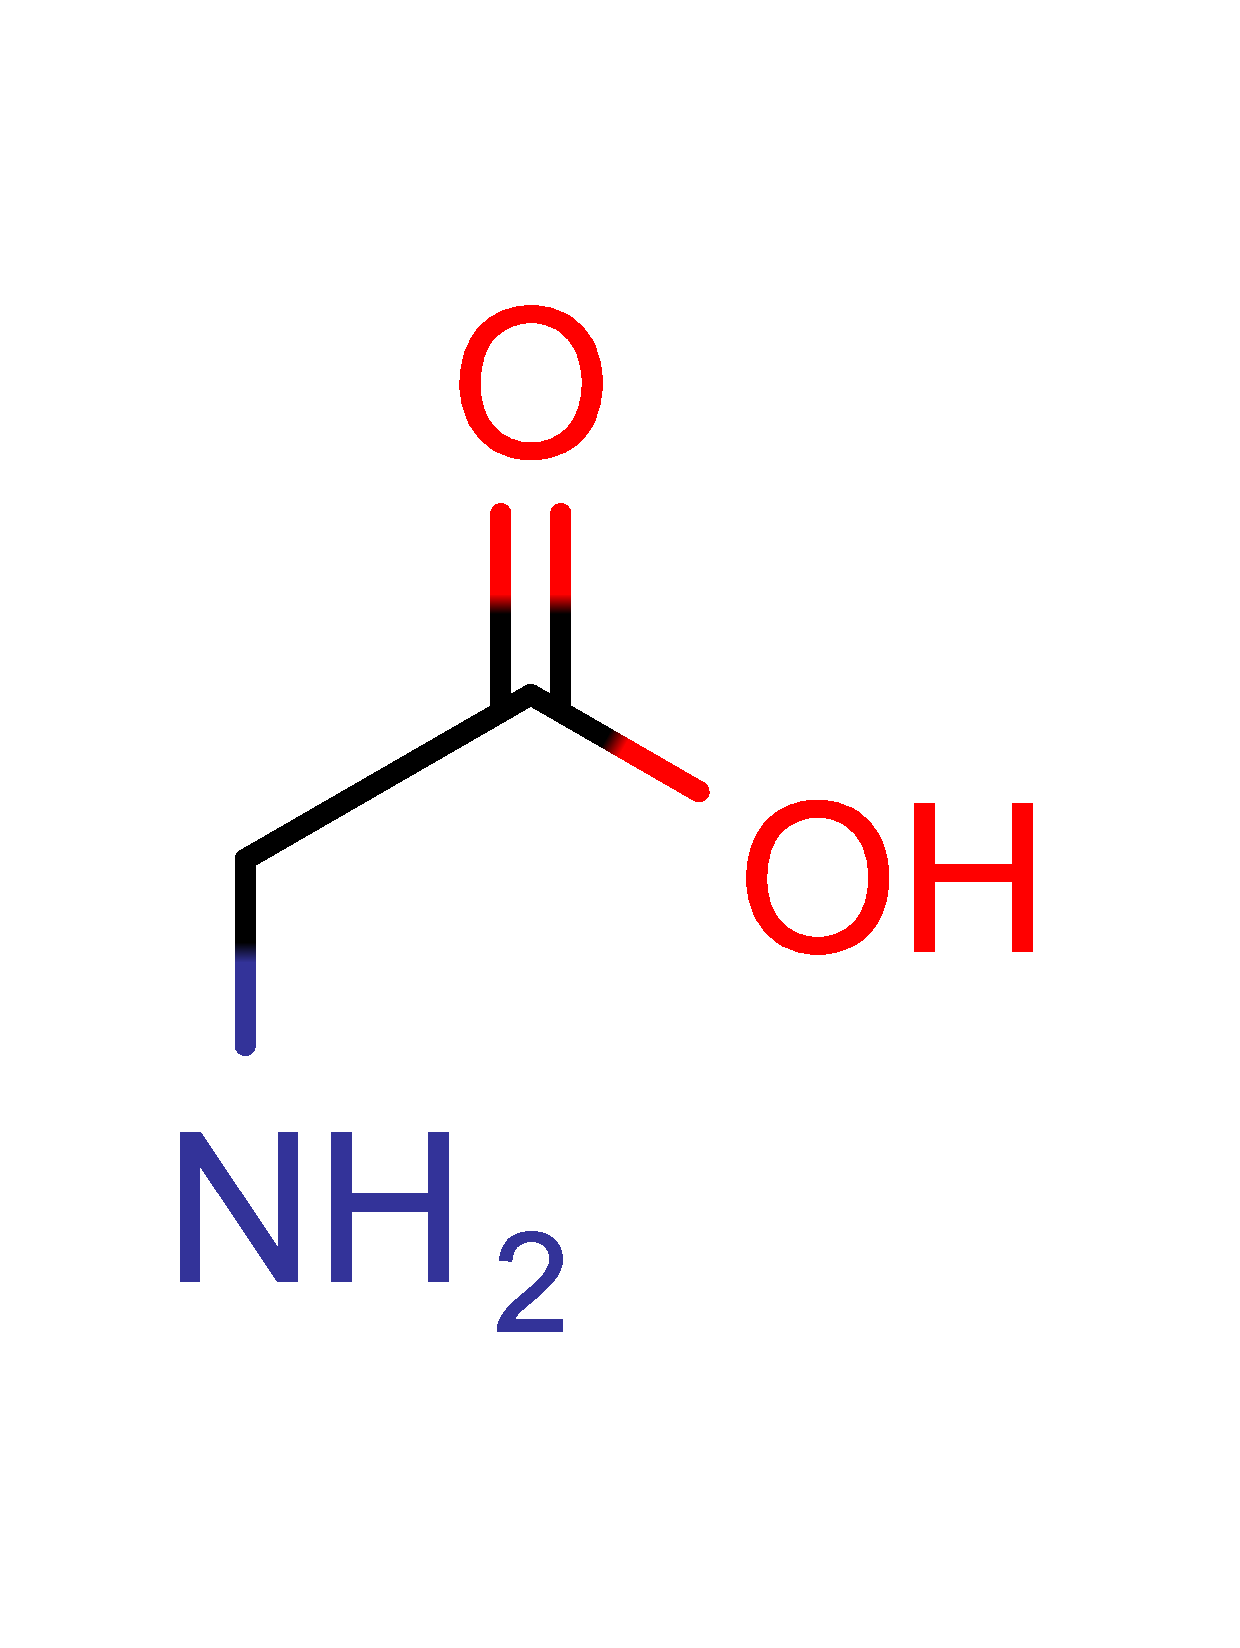
\includegraphics[width=0.3\linewidth]{images/Glicina}
		\caption{Estructura qu\'imica de la glicina.}
		\label{fig:glicina}
	\end{scheme}
	
	La bioinorg\'anica del n\'iquel tambi\'en tiene sus pecularidades, dado que fue el \'unico metal de transici\'on con periodo 3 al que no se le hab\'ian atribu\'ido funciones biol\'ogicas para 1975. Lo anterior se debi\'o en parte a que el n\'iquel no presenta bandas de absorci\'on caracter\'isticas al coordinarse con ligandos biol\'ogicos. La perspectiva biol\'ogica del n\'iquel cambi\'o al descubrirse que la ureasa es una enzima de este metal \cite{Nickel}. 
	
	En general, el n\'iquel al igual que la mayor\'ia de metales de transici\'on prefiere una geometr\'ia octa\'edrica. Por esta raz\'on se tiene un n\'umero m\'aximo de coordinaci\'on 6, sin embargo como el glicinato act\'ua como un ligando bidentado, es posible alcanzar \'unicamente tres diferentes iones en soluci\'on con constantes de equil\'ibrio $K_1$, $K_2$ y $K_3$, los cuales se muestran en la \autoref{fig:ligands}.
	
	\scriptsize
	\begin{equation}\label{eq: constants}
	\def\arraystretch{3}
		\begin{array}{cc}
			\ce{Ni^{2+} + Gly- <=> Ni(Gly)+} & K_1 = \dfrac{\ce{[Ni(Gly)+]}}{\ce{[Ni^{2+}][Gly^-]}}\\
			\ce{Ni(Gly)+ + Gly- <=> Ni(Gly)_2} & K_2 = \dfrac{\ce{[Ni(Gly)_2]}}{\ce{[Ni(Gly)+][Gly^-]}}\\
			\ce{Ni(Gly)_2 + Gly- <=> Ni(Gly)_3-} & K_3 = 		\dfrac{\ce{[Ni(Gly)_3^-]}}{\ce{[Ni(Gly)_2][Gly^-]}}
		\end{array}
	\end{equation}
	\normalsize
	
	Con el objetivo de facilitar los c\'alculos posteriores se introducen las constantes de equilibrio globales:
	\begin{equation}
		\beta_n = \prod\limits_{i=1}^{i \leq n} K_i
	\end{equation}
	
	Usando el m\'etodo de J. Bjerrum es posible calcular las constantes globales conociendo la relaci\'on entre las moles de glicinato ligado y el cati\'on libre.
	\small  
	\begin{equation}\label{eq: fit}
	\def\arraystretch{3}
		\begin{array}{rl}
			\tilde{n} & = \dfrac{\ce{\beta_1[Gly^-] + 2\beta_2[Gly^-]^2 + 3\beta_3[Gly^-]^3}}{\ce{1 + \beta_1[Gly^-] + \beta_2[Gly^-]^2 + \beta_3[Gly^-]^3}} \\
			& = \dfrac{\ce{[Gly]}_0 - (1+K_a/\ce{[H+]})(C_H + \ce{[OH^-] - [H+]})}{\ce{[NiCl2]}_0}
		\end{array}
	\end{equation}
	\normalsize
	
	Donde $K_a$ es la constante de acidez de la glicina, $C_H$ la concentraci\'on de protones debido al \'acido n\'itrico, y el factor $K_a/\ce{[H+]}(\cdots)$ corresponde con la concentraci\'on de glicina libre \ce{[Gly^-]}. Reescribiendo la ecuaci\'on se obtiene:
	\footnotesize
	\begin{equation}\label{eq: Rossetti}
	\dfrac{\tilde{n}}{(1-\tilde{n})\ce{[Gly^-]}} = \beta_1 + \dfrac{(2-\tilde{n})}{(1-\tilde{n})}\ce{[Gly^-]}\beta_2 + \dfrac{(3-\tilde{n})}{(1-\tilde{n})}\ce{[Gly^-]}^2\beta_3
	\end{equation}
	\normalsize
	
	\begin{figure*}[h]
		\centering
		\begin{tabular}{ccc}
			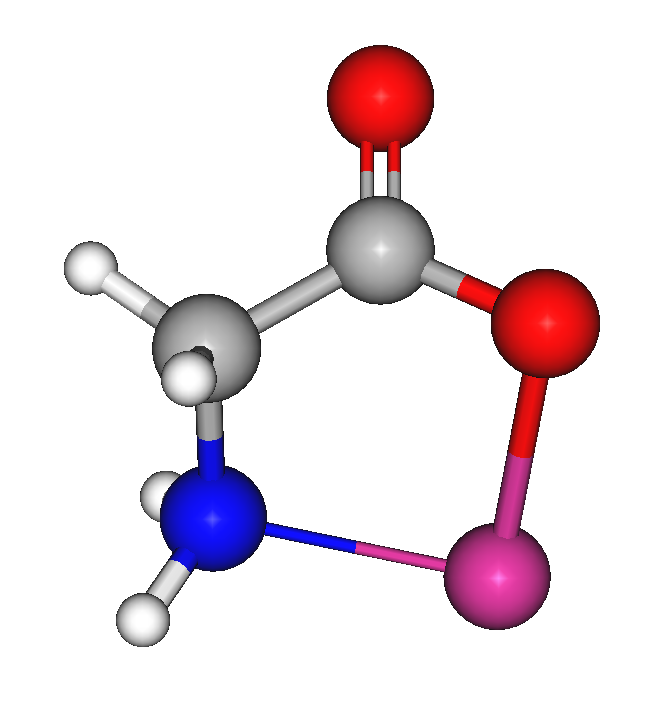
\includegraphics[width=0.2\linewidth]{images/Single.png} & 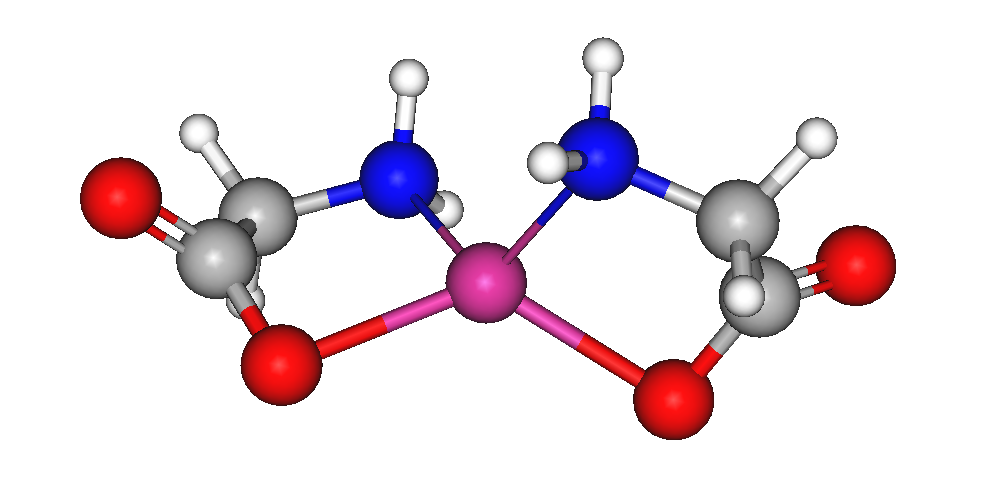
\includegraphics[width=0.4\linewidth]{images/Double.png} &
			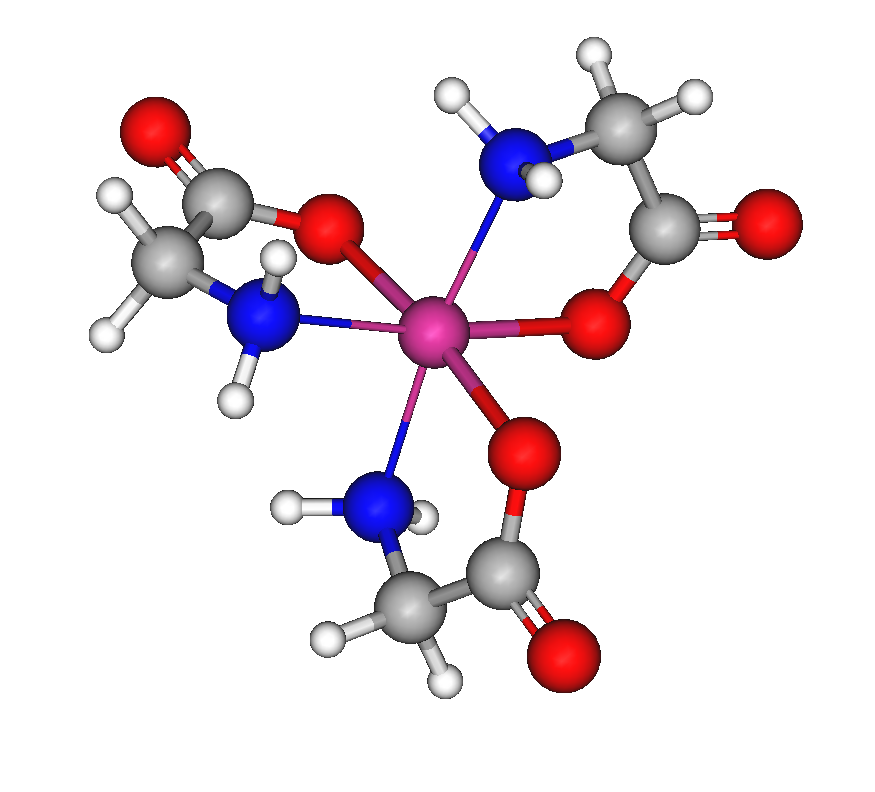
\includegraphics[width=0.3\linewidth]{images/Triple.png}
		\end{tabular}
		\caption{Distintos complejos de glicinato de n\'iquel en soluci\'on. Las esf\'eras rojas representan ox\'igenos, en gris se muestran los carbonos, hidr\'ogenos en blanco, y los \'atomos de nitr\'ogeno en azul.}
		\label{fig:ligands}
	\end{figure*} 
	
	Para la realizaci\'on del an\'alisis se toman dos aproximaciones importantes. En primer lugar el coeficiente de actividad $\gamma$ se asume constante a lo largo del experimento dado que la contribuci\'on de los iones distintos al nitrato es despreciable, pues estos u\'ltimos se trabajan con al menos tres \'ordenes de magnitud menos.
	\begin{equation}
	\ce{[H+]} = \dfrac{10^{-pH}}{\gamma_\pm}
	\end{equation}
	
	En segundo lugar las concentraciones iniciales de glicinato y n\'iquel se asumen constantes a lo largo del experimento, esto debido a que el cambio neto de volumen no supera el 5 \% del volumen inicial.
	
	
	\section{Metodolog\'ia}
	Una soluci\'on de 100 mL de NaOH es preparada a partir de 2.000 g de la base s\'olida, la soluci\'on se estandariza usando 5 mL de NaOH en 0.511 g de ftalato \'acido de potasio. Se establece la concentraci\'on de la soluci\'on en 0.5 M. Usando  16 mL de NaOH (0.5 M) y 0.6005 g de glicina se obtiene el glicinato de sodio, que posteriormente es aforado a 20 mL.
	
	Usando un beaker se prepara una soluci\'on que contiene 0.241 g de \ce{NiCl_2.6H_2O}, 10 mL de \'acido n\'itrico $0.11\pm0.1$ M, 100 mL de una soluci\'on de nitrato de potasio previamente preparada con concentraci\'on 0.2015 M, y 90 mL de agua. Con una bureta se adicionan al\'icuotas de 0.2 mL de glicinato de sodio a la soluci\'on hasta completar 10 mL.
	
	\section{Resultados y Discusi\'on}
	
	Los resultados obtenidos usando la titulaci\'on potenciom\'etrica se muestran en la \autoref{fig: pH}. Es necesario tener en cuenta que el pH corresponde con la actividad del hidr\'ogeno en soluci\'on, raz\'on por lo cual se debe conocer la fuerza i\'onica en soluci\'on.
	\begin{equation}\label{eq: strength}
		\mu = \dfrac{1}{2}\sum\limits_{i=1}^{3} M_iZ_i^2
	\end{equation}
	\pagebreak
	
	\begin{figure}[h]
		\centering
		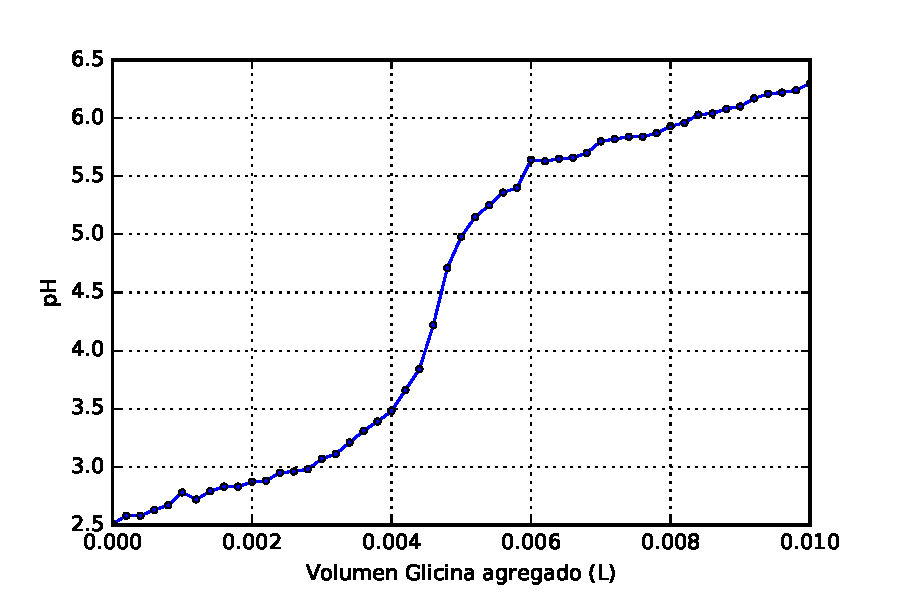
\includegraphics[width=\linewidth]{images/pH.pdf}
		\caption{Resultados obtenidos para la titulaci\'on de la glicina en soluci\'on con Ni(II).}
		\label{fig: pH}
	\end{figure}
	
	La fuerza i\'onica se calcula a partir de la concentraci\'on de las esp\'ecies i\'onicas en soluci\'on y su carga. En este caso el nitrato de potasio, el cloruro de n\'iquel y el \'acido n\'itrico. La fuerza i\'onica a su vez permite conocer el coeficiente de actividad del hidr\'ogeno $\gamma_\pm$ haciendo uso de la ecuaci\'on de Debye–H\"uckel:
	\begin{equation}\label{eq: activity}
		-\log\gamma_\pm = \dfrac{Z_1 Z_2 \sqrt{\mu}}{2\left(1+\sqrt{\mu}\right)}
	\end{equation}
	
	Usando las \autoref{eq: strength} y \autoref{eq: activity} se obtiene la concentraci\'on de protones en la soluci\'on. El coeficiente de actividad promedio, junto con la fuerza i\'onica se muestran en la \autoref{fig: versus}, adem\'as de la relaci\'on entre \ce{[H^+]} y \ce{[OH^{-}]}, los \'ultimos son obtenidos usando la constante de autoionizaci\'on del agua a $\mu = 0.1$ M:
	\begin{equation}
		\def\arraystretch{2}
		\begin{array}{rl}
			\ce{[H+]} = & \dfrac{10^{-pH}}{\gamma_\pm} = 10^{\left(\frac{Z_1Z_2\sqrt{\mu}}{2\left(1+\sqrt{\mu}\right)} - pH\right)} \\
			\ce{[OH^{-}]} = & \dfrac{K_w}{\ce{[H+]}}
		\end{array}
	\end{equation}
	
	\begin{figure*}[h]
		\centering
		\begin{tabular}{cc}
			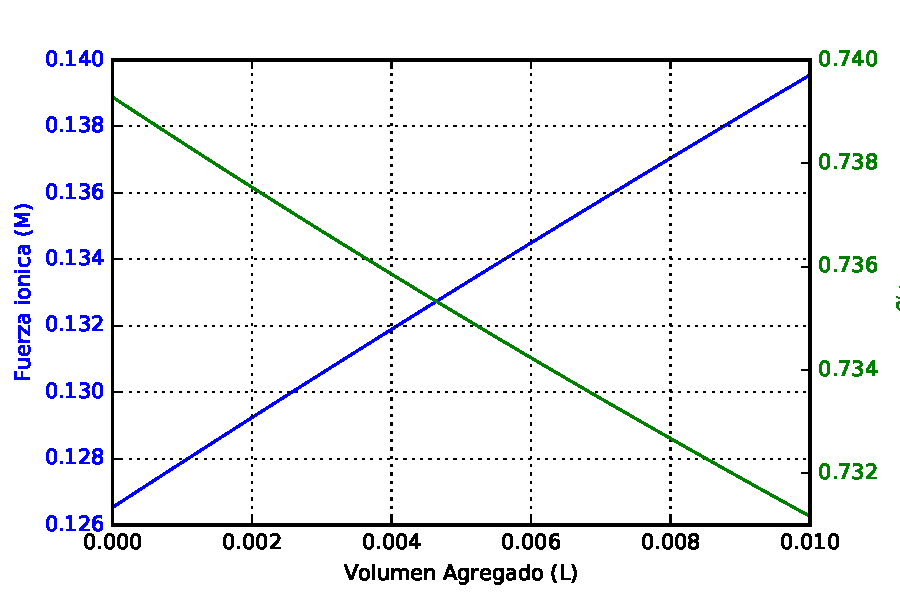
\includegraphics[width=0.5\linewidth]{images/ionic_strength.pdf} & 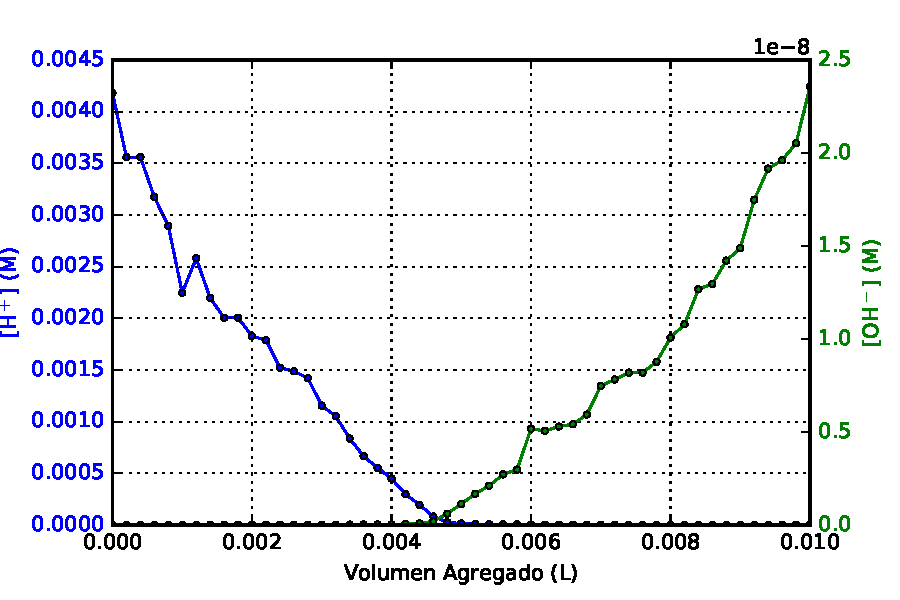
\includegraphics[width=0.5\linewidth]{images/HOH.pdf}
		\end{tabular}
		\caption{A la izquierda, relaci\'on entre la fuerza i\'onica, y el coeficiente de actividad promedio en funci\'on del volumen agregado. A la derecha se encuentra la relaci\'on entre los protones en soluci\'on y los iones hidroxilos en funci\'on del volumen de glicina.}
		\label{fig: versus}
	\end{figure*}
	\pagebreak
	
	En la \autoref{fig: versus} se observa que la variaci\'on m\'axima de la fuerza i\'onica es de cerca del 11 \%, raz\'on por la cual se recomienda calcular el valor de la misma para cada adici\'on de glicina a la soluci\'on.
	\begin{figure}[h]
		\centering
		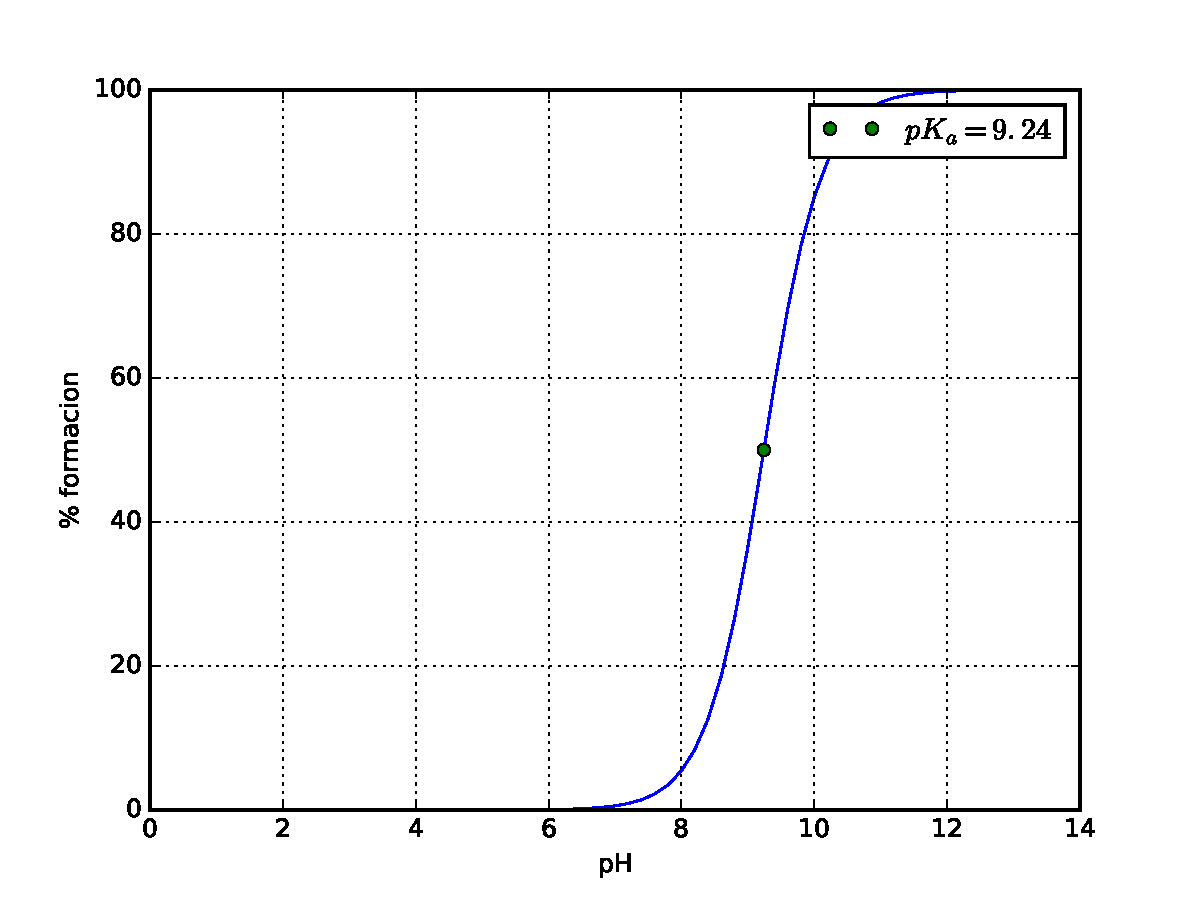
\includegraphics[width=\linewidth]{images/pka_sim.pdf}
		\caption{Simulaci\'on de la constante de acidez de la glicina.}
	\end{figure}
	
	Como fue discutido en la introducci\'on existen dos m\'etodos distintos para calcular las constantes de equilibrio de los complejos de glicinato de n\'iquel. Ambos se derivan de la \autoref{eq: fit} que depende de la constante de acidez de la glicina. Dado que este valor no se midi\'o experimentalmente, se llev\'o a cabo una simulaci\'on. Los puntos obtenidos fueron usados en una interpolaci\'on c\'ubica con el objetivo de encontrar el valor de pH para el cual el porcentaje de formaci\'on corresponde con 50 \%. Los datos de la simulaci\'on, los datos experimentales y la totalidad del algoritm\'o usado en el an\'alisis de los datos se encuentran disponibles en \href{https://github.com/jsbarbosa/study-happiness/tree/master/Lab\%20Inorganica/7-Aminoacidos}{\color{blue}GitHub} \footnote{https://github.com/jsbarbosa/study-happiness/tree/master/Lab\%20Inorganica/7-Aminoacidos}.
	
	Para el m\'etodo de Bjerrum, tambi\'en es necesario realizar una interpolaci\'on de los datos con el objetivo de obtener los valores exactos para los cuales \ce{[Gly^{-}]} da lugar a $\tilde{n} = 1/2, 3/2, 5/2$, como se muestra en la \autoref{fig: Bjerrum}, siendo estos valores aproximados para relaciones de metal ligando 1:1, 1:2 y 1:3 en el complejo. Usando la \autoref{eq: constants} y la relaci\'on metal - ligando se obtiene:
	\begin{equation}
		K_i = \dfrac{1}{\ce{[Gly^-]}(\tilde{n} = (2i-1)/2)^i}
	\end{equation}
	
	\begin{figure}[h]
		\centering
		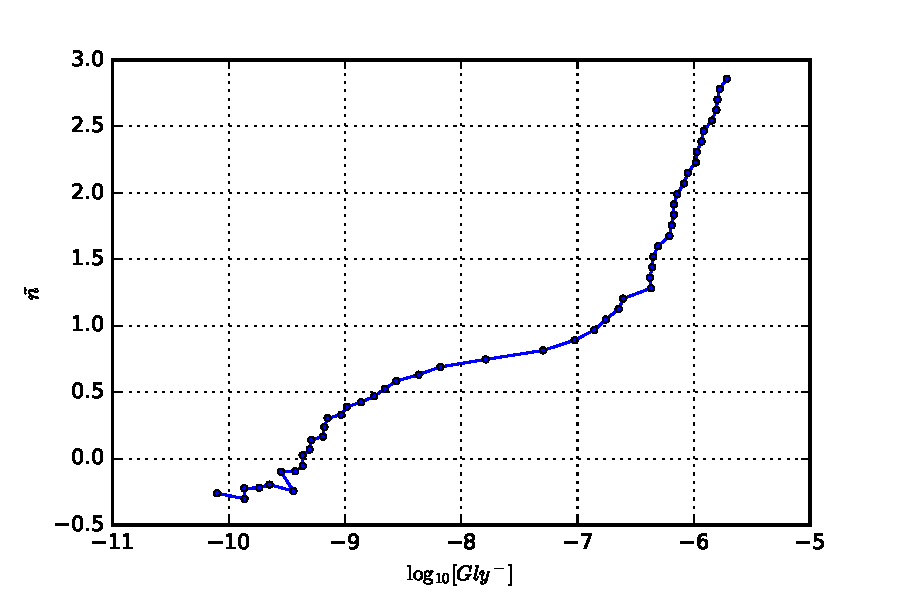
\includegraphics[width=\linewidth]{images/Bjerrum.pdf}
		\caption{Relaci\'on entre las moles de glicinato ligado y n\'iquel en soluci\'on en funci\'on de la concentraci\'on de glicinato en soluci\'on.}
		\label{fig: Bjerrum}
	\end{figure}
	
	\begin{figure*}[h]
		\centering
		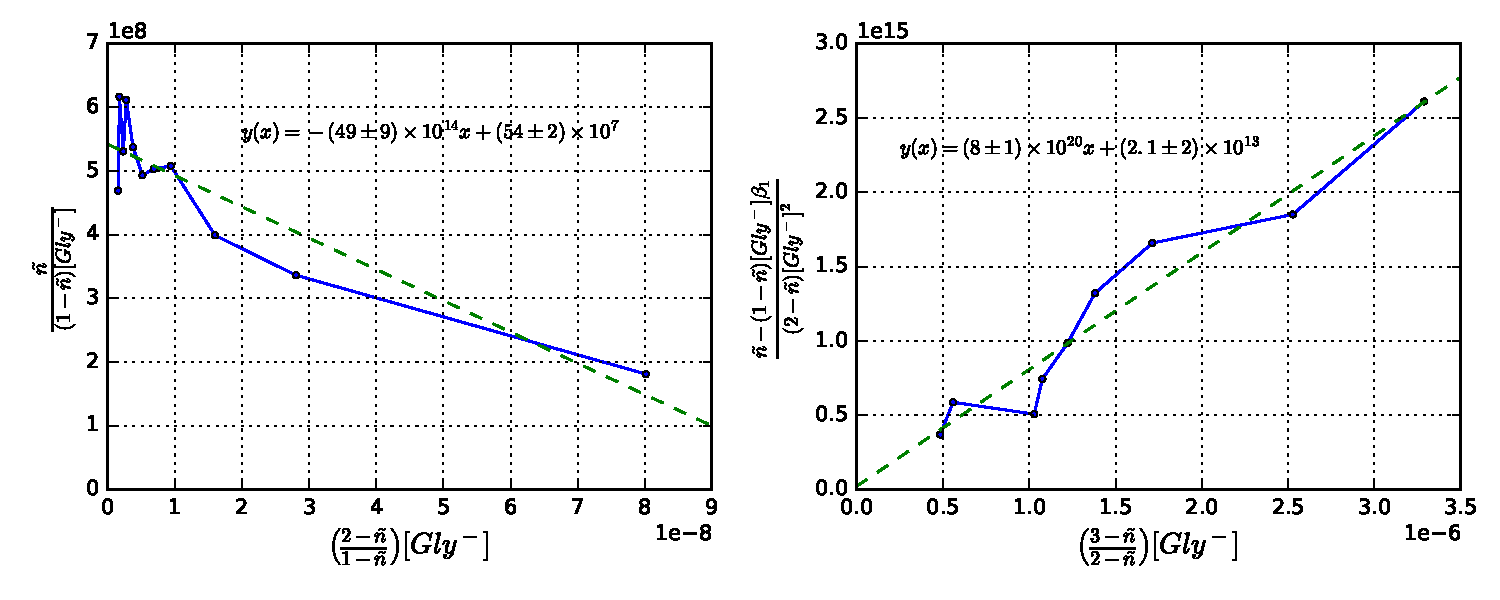
\includegraphics[width=\linewidth]{images/Rossotti.pdf}
		\caption{Regresiones propias del m\'etodo de Rossetti. En la gr\'afica izquierda se muestra la funci\'on truncada al primer orden, a la derecha los t\'erminos de \'orden superior.}
		\label{fig: Rossetti}
	\end{figure*}
	
	Los valores obtenidos para las constantes se muestra en la \autoref{tb: Bjerrum}. En ella se puede observar un resultado aparentemente contradictorio en la forma como se comporta el n\'iquel en presencia de glicinato, puesto que se obtiene $K_3 > K_2 > K_1$.
	\pagebreak
	
	\begin{table}[h]
		\centering
		\caption{Constantes de equilibrio obtenidas por el m\'etodo de Bjerrum.}
		\begin{tabular}{cc}
			\hline
			 & $K_i$ (M$^{-1}$) \\
			\hline
			$K_1$ & $4.99\times10^{8}$ \\
			$K_2$ & $5.03\times10^{12}$ \\
			$K_3$ & $4.48\times10^{17}$ \\
			\hline
		\end{tabular}
		\label{tb: Bjerrum}
	\end{table}
	
	En el caso del modelo de Rossetti se usa la \autoref{eq: Rossetti}, asumiendo que $K_1 \gg K_2 \gg K_3$ es posible truncar la funci\'on para calcular el t\'ermino de primer orden. Una vez calculado este valor es posible calcular el t\'ermino de segundo y tercer orden. Este proceso se muestra en la \autoref{fig: Rossetti}, del intercepto de la primera gr\'afica es posible extraer $\beta_1 = K_1$, de la segunda gr\'afica el intercepto corresponde con $\beta_2$ y la pendiente con $\beta_3$.
	\begin{table}[h]
		\centering
		\caption{Constantes de equilibrio obtenidas por el m\'etodo de Rossetti.}
		\begin{tabular}{cc}
			\hline
			& $K_i$ (M$^{-1}$) \\
			\hline
			$K_1$ & $(5.4\pm 0.2)\times10^{8}$ \\
			$K_2$ & $(3.8\pm 3.6)\times10^{4}$ \\
			$K_3$ & $(3.7\pm 0.5)\times10^{7}$ \\
			\hline
		\end{tabular}
		\label{tb: Rossetti}
	\end{table}
	
	Los resultados obtenidos con el m\'etodo de Rossetti son a\'un m\'as contradictorios, pues se obtiene $K_1 > K_3 \gg K_2$. En este sentido a pesar de que el m\'etodo de Bjerrum constituye un m\'etodo aproximado, no depende de que el orden de las constantes de equilibrio sea descendiente, aunque tiene la ventaja de proveer la incertidumbre del m\'etodo. 
	
	Sin embargo el orden de las constantes de equilibrio obtenidas por el m\'etodo de Bjerrum a\'un carece de explicaci\'on. Si se tiene en cuenta la \autoref{eq: constants} se puede observar que constantes de equilibrio m\'as grandes implican que la reacci\'on se ve desplazada hacia los productos. En este sentido que la constante de equilibrio $K_3$ sea mayor a $K_2$ y $K_1$, sugiere un probable efecto quelato. A la luz de los resultados se cree que la naturaleza del n\'iquel en soluci\'on es tal que para 3 ligandos glicinato libres, el n\'iquel preferir\'a que un s\'olo cati\'on se coordine con todos ellos a que estos se repartan uniformemente. Lo anterior siendo consecuencia del efecto quelato.

	\section{Preguntas}
	\subsection{Dibujar todos los is\'omeros \'opticos y geom\'etricos de los tres complejos de}
	\subsubsection{\ce{[Ni(Gly^-)]^+}}
	\begin{figure}[h]
		\centering
		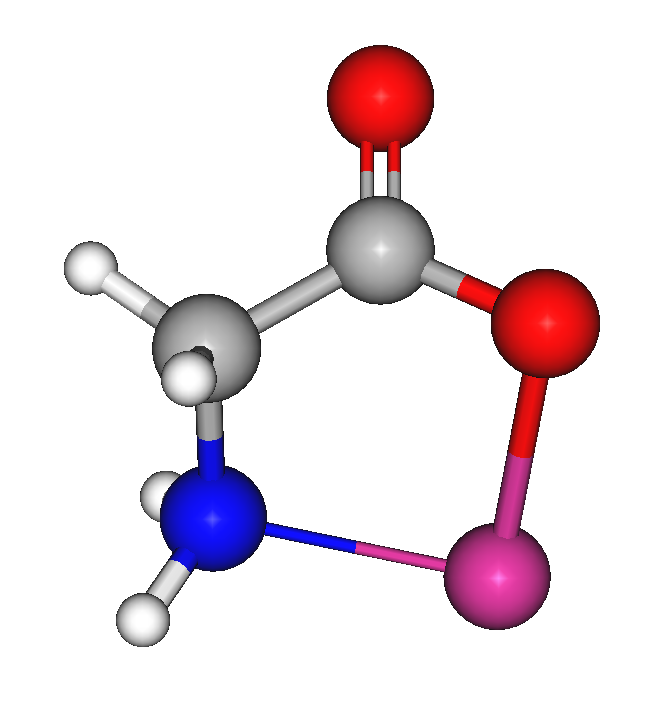
\includegraphics[width = 0.4\linewidth]{images/Single.png}
		\caption{\'Unico is\'omero posible}
	\end{figure}
	
	\subsubsection{\ce{[Ni(Gly^-)_2]}}
	\begin{figure}[h]
		\centering
		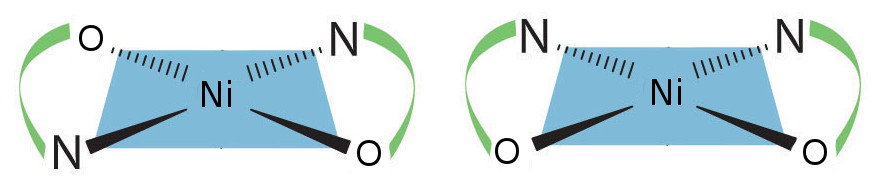
\includegraphics[width = \linewidth]{images/cis_trans.jpg}
		\caption{Is\'omeros trans y cis.}
	\end{figure}
	
	\pagebreak
	\subsubsection{\ce{[Ni(Gly^-)_3]^-}}
	\begin{figure}[h!]
		\centering
		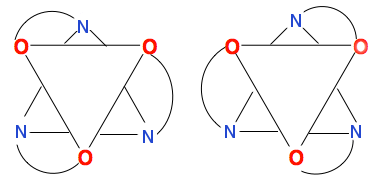
\includegraphics[width = 0.7\linewidth]{images/delta_lambda.png}
		\caption{Is\'omero $\delta$ y $\Lambda$}
	\end{figure}
	
	\subsection{Derivar la ecuaci\'on 11}
	La glicina se deprotona dando lugar a la siguiente reacci\'on:
	\begin{equation}\label{Ka}
	\begin{array}{lr}
	\ce{Gly ->[K_a] H+ + Gly^-} & K_a = \dfrac{\ce{[H+][Gly^-]}}{\ce{[Gly]}}
	\end{array}
	\end{equation}
	
	Aplicando logaritmo a ambos lados y multiplicando por -1 es obtiene una ecuaci\'on para el $pKa$.
	\begin{equation}\label{pKa}
	pK_a = -\log K_a = -\log\ce{[H+]} - \log\left(\dfrac{\ce{[Gly^-]}}{\ce{[Gly]}}\right)
	\end{equation}
	
	Considerando la conservaci\'on de carga en la soluci\'on:
	\begin{equation}
	\ce{[Gly^-]} = \ce{[H+] + [Na+] - [OH^-]}
	\end{equation}
	
	Aplicando conservaci\'on de la masa:
	\footnotesize
	\begin{equation}
	\ce{[Gly]} = \ce{[Gly_0]-[Gly^-]} = \ce{[Gly_0]} - \left(\ce{[H+] + [Na+] - [OH^-]}\right)
	\end{equation}
	\normalsize
	
	\small
	Reemplazando las ecuaciones anteriores en la \autoref{pKa}.	
	\begin{equation*}
	pKa = -\log\ce{[H+]} - \log\left(\dfrac{\ce{[H+] + [Na+] - [OH^-]}}{\ce{[Gly_0]} - \left(\ce{[H+] + [Na+] - [OH^-]}\right)}\right)
	\end{equation*}
	\normalsize
	
	\subsection[Se prepara]{Se prepara una disoluci\'on por mezclar de 100 mL de glicina (0.2 M) y 100 mL de \ce{Cu^{2+}} (0.2 M), el pH se ajust\'o a 7 con una soluci\'on de NaOH. Calcule los porcentajes aproximados del ion \ce{Cu^{2+}} original, as\'i como los actuales despu\'es de efectuar la mezcla, \ce{Cu^{2+}}, \ce{CuA+}, y \ce{CuA_2} en la soluci\'on. Use $pK_a$ de 9.60 para la glicina y las siguientes constantes de estabilidad:}
	\begin{equation*}
	\begin{array}{lcrc}
	\ce{Cu^{2+} + A-} & \ce{<=>} & \ce{CuA+} & \log K_1 = 8.38\\
	\ce{CuA+ + A-} & \ce{<=>} & \ce{CuA_2} & \log K_2 = 6.87 
	\end{array}
	\end{equation*}
	
	Usando las constantes de equilibrio:
	\begin{equation}
	\def\arraystretch{3}
	\begin{array}{cc}
	K_a = \dfrac{\ce{[A^-][H+]}}{\ce{[HA]}} & \log K_a = 9.60 \\
	K_1 = \dfrac{\ce{[CuA+]}}{\ce{[Cu+2][A^-]}} & \log K_1 = 8.38 \\
	K_2 = \dfrac{\ce{[CuA_2]}}{\ce{[CuA+][A^-]}} & \log K_2 = 6.87 \\
	\end{array}
	\end{equation}
	
	Sustituyendo en las concentraciones de cobre de obtiene:
	\begin{equation}
	\begin{array}{c}
	\ce{[CuA+]} = \ce{K_1K_a}\dfrac{\ce{[Cu^{+2}][HA]}}{\ce{[H+]}}\\
	\ce{[CuA_2]} =  \ce{K_2K_1K_a^2}\dfrac{\ce{[Cu^{+2}][HA]^2}}{\ce{[H+]^2}}
	\end{array}
	\end{equation}
	
	Teniendo en cuenta las leyes de conservaci\'on:
	\begin{equation}
	\begin{array}{cc}
	\ce{[Cu^{2+}]_0} = \ce{[Cu^{+2}] + [CuA+] + [CuA_2]} \\
	\ce{2[Cu^{2+}] + [CuA+] + [H+]} = \ce{[A^-] + [Cl^-]}
	\end{array}
	\end{equation}
	
	\subsection{Se desea determinar las constantes de formaci\'on ($K_1$, $K_2$ y $K_3$) para los complejos de coordinaci\'on de etilendiamina, a \ce{Ni^{2+}} formando los complejos \ce{[Ni(en)]^{2+}}, \ce{[Ni(en)_2]^{2+}}, \ce{[Ni(en)_3]^{2+}}}
	\subsubsection{C\'omo determinar\'ia el primer y segundo $pKa$ de la etilendiamina?}
	Es posible obtener los valores de $pKa$ usando una titulaci\'on potenciom\'etrica. A partir de los valores obtenidos se puede calcular num\'ericamente los puntos de inflexi\'on de las curvas usando segundas derivadas \cite{pka determination}.
	
	\subsubsection{Defina estos dos valores de $pKa$. ?`Cu\'al de los dos ser\'ia el m\'as grande?}
	Sean $Ka_1$ y $Ka_2$ las constantes de acidez de la etilendiamina, donde $Ka_1$ es la de menor valor. Existen dos posibles posiciones de protonaci\'on debido al pH. Existen entonces 3 regiones: a pH b\'asico donde la etilendiamina se encuentra en su forma molecular ($pKa_2$), una regi\'on intermedia en donde una de las dos aminas tiene carga y la \'ultima a pH \'acido donde las dos aminas estar\'an protonadas ($pKa_1$).
	\begin{scheme}[h]
		\centering
		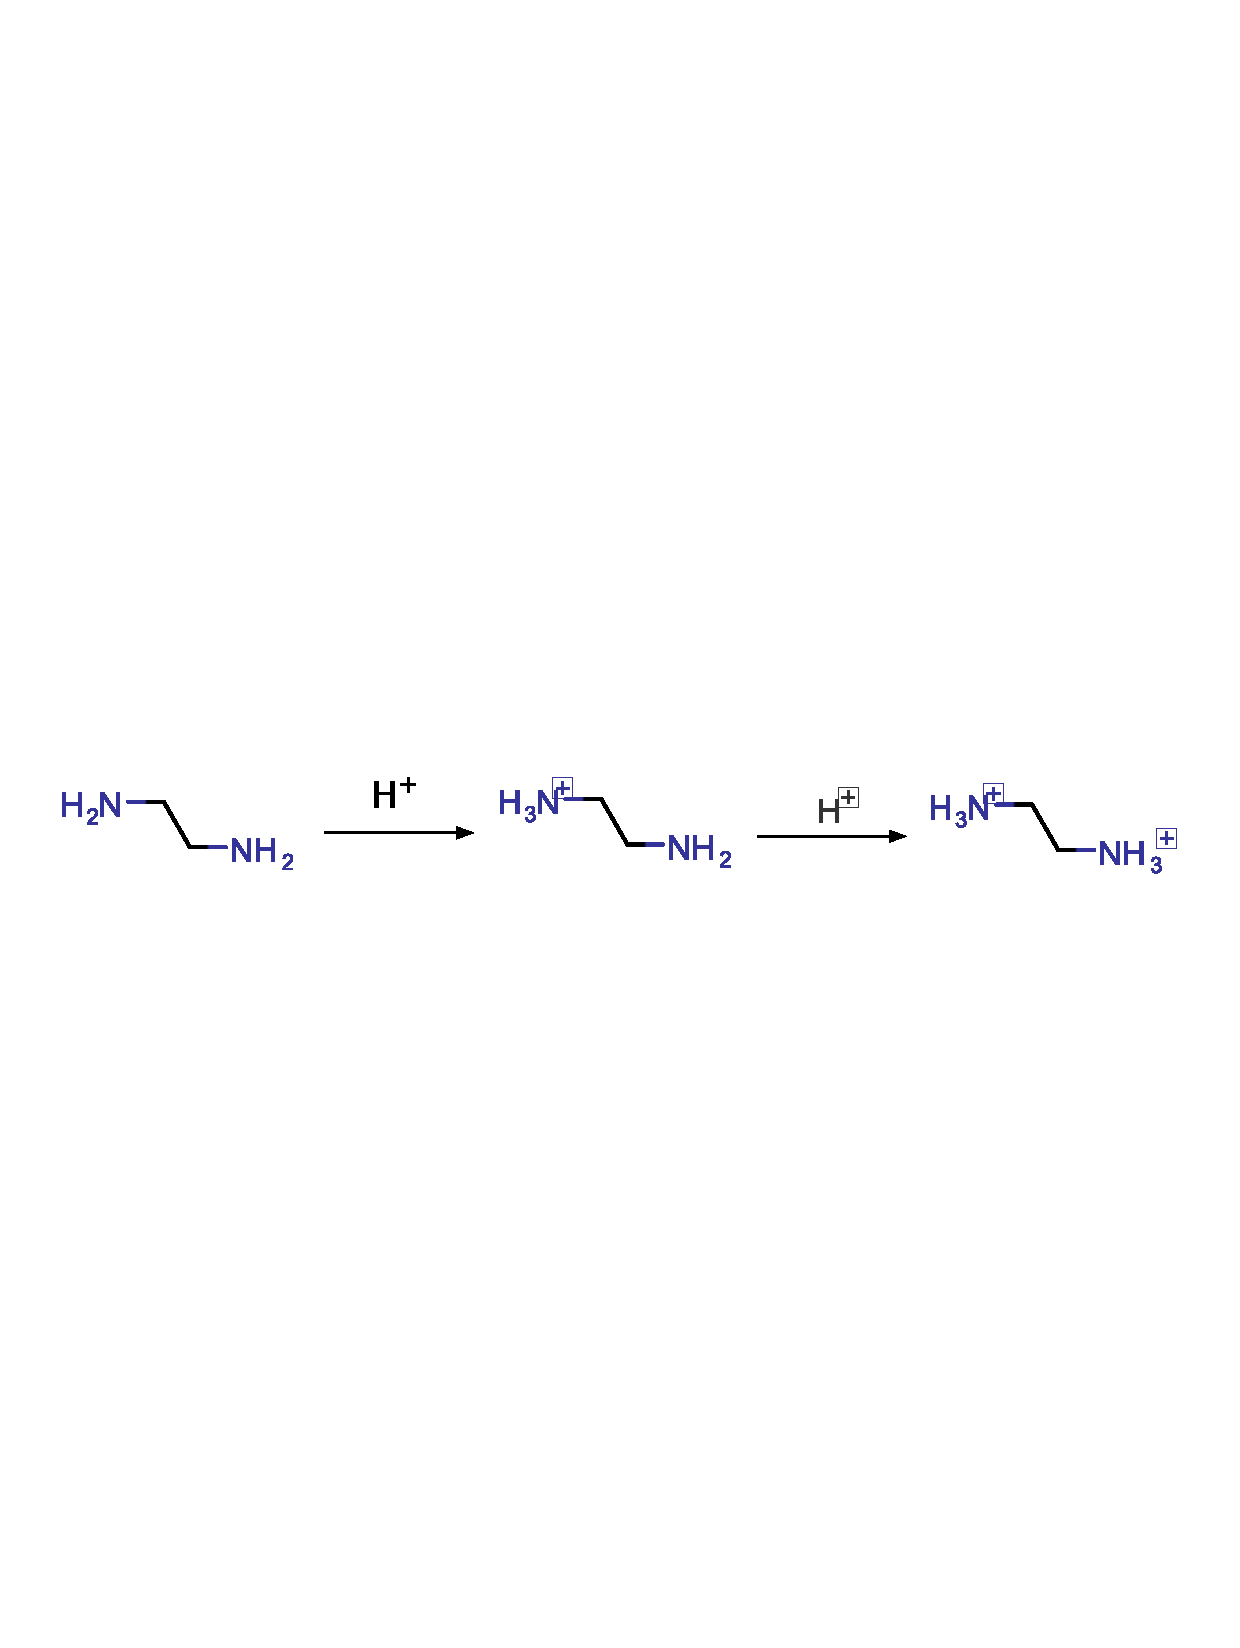
\includegraphics[width=\linewidth]{images/en_pKa.pdf}
		\caption{Posibles estructuras de la etilendiamina dependiendo del pH.}
		\label{sch:etilen_pka}
	\end{scheme}
	
	\subsubsection{Cu\'ales titulaciones realizar\'ia para determinar las constantes de estabilidad $K_1$, $K_2$ y $K_3$? Explique brevemente. El procedimiento difiere de lo utilizado en este experimento?}
	Es posible realizarlo de la misma forma siendo el an\'alisis posterior basado en el m\'etodo de J. Bjerrum, adicionalmente es posible obtener informaci\'on sobre la estructura del complejo usando una titulaci\'on y posterior determinaci\'on en UV-vis, siendo el segundo m\'etodo recomendado para concentraciones m\'as bajas \cite{pka determination}.
	
	\subsubsection{Qu\'e valor esperar\'ia sea m\'as grande, el de $K_1$ o el de $K_2$?}
	Debido a que la facilidad de acomplejamiento con el metal depende de la carga del cati\'on, se espera la misma dependencia que se observa con los complejos de glicinato de n\'iquel. De esta forma $K_1 > K_2$.
	
	\section{Conclusiones}
	Dos m\'etodos distintos fueron usados para calcular los valores de las constantes de equilibrio para los complejos con glicinato de n\'iquel. El an\'alisis de los resultados presentados por los m\'etodos sugiere al m\'etodo de Bjerrum como m\'as preciso debido a los valores obtenidos para las constantes de equilibrio, $K_1 = 4.99\times10^8$, $K_2 = 5.03\times10^{12}$, $K_3 = 4.48\times10^{17}$ M$^{-1}$. El orden presentado por las constantes es atribu\'ido a el efecto quelato presentado por los ligandos glicinato. Para ambos m\'etodos se logra establecer que los complejos de glicinato de n\'iquel presentan una estabilidad considerable con constantes de equilibrio con $pK > 4$.
	
	\phantomsection
	\bibliographystyle{unsrt}
	\begin{thebibliography}{9}
		\bibitem{Glycine}
		\textit{Glycine}; Encyclopedic Reference of Genomics and Proteomics in Molecular Medicine; Springer Berlin Heidelberg: Berlin. Heidelberg, 2006; pp 703.
		\bibitem{GlycineHistory}
		\textit{Glycine}; Encyclopedia of Astrobiology; Springer Berlin Heidelberg: Berlin. Heidelberg, 2015; pp 994.
		\bibitem{Nickel}
		Kaim, W.; Schwederski, B.; Klein, A. \textit{Bioinorganic chemistry: Inorganic elements in the chemistry of life - an introduction and guide}, 2nd ed.; Wiley-Blackwell (an imprint of John Wiley \& Sons Ltd): Oxford, United Kingdom, \textbf{2011}; p 300.
		\bibitem{pka determination}
		Babi\'c, S.; Horvat, A. J. M.; Mutavdzic Pavlovic, D.; Kastelan-Macan, M. Determination of pKa values of active pharmaceutical ingredients. \textit{TrAC Trends in Analytical Chemistry}. Published Online: Dec 2007, 26 (\textit{11}), 1043–1061.
	\end{thebibliography}
\end{document}